\documentclass[border=4pt]{standalone}
\usepackage{tikz}
\usetikzlibrary{arrows,positioning}
\begin{document}
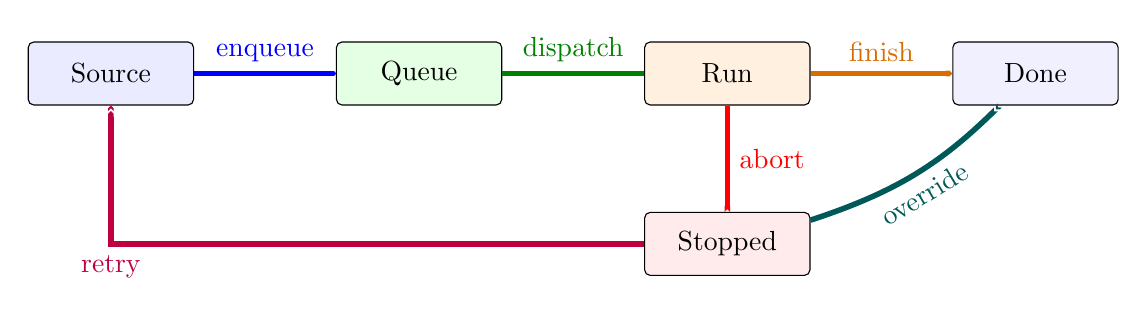
\begin{tikzpicture}[
  node distance=1.35cm and 1.8cm,
  stage/.style={draw,rounded corners=2pt,minimum width=2.1cm,minimum height=8mm,align=center}
]
  \node[stage,fill=blue!8] (source) {Source};
  \node[stage,fill=green!10,right=of source] (queue) {Queue};
  \node[stage,fill=orange!12,right=of queue] (run) {Run};
  \node[stage,fill=blue!6,right=of run] (done) {Done};
  \node[stage,fill=red!8,below=of run] (stop) {Stopped};

  \draw[blue,line width=2pt,-{round cap}] (source) -- node[above]{enqueue} (queue);
  \draw[green!50!black,line width=2pt,-{butt cap}] (queue) -- node[above]{dispatch} (run);
  \draw[orange!85!black,line width=2pt,-{triangle 90 cap}] (run) -- node[above]{finish} (done);
  \draw[red,line width=2pt,-{triangle 90 cap reversed}] (run) -- node[right]{abort} (stop);
  \draw[purple,line width=2pt,-{fast cap}] (stop) -| node[below]{retry} (source);
  \draw[teal!70!black,line width=2pt,-{fast cap reversed}] (stop) to[bend right=13] node[below,sloped]{override} (done);
\end{tikzpicture}
\end{document}
